\section{New Method}


\begin{figure*}[htb]
\centering
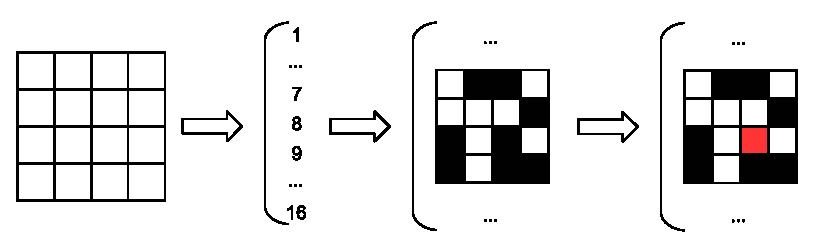
\includegraphics[width=0.8\textwidth]{fig/brute_force.eps}
\caption{some figure}
\end{figure*}


This work aims to find the optimal number and distribution of light cores for a fixed set of cores to achieve the maximum performance-per-watt, with consideration of thermal constraints. In order to estimate the power consumption of a multi-core system for different number of light cores and various light core distributions, we first propose an iteration based full-chip power estimation method with brute force search static, which is accurate but very time-consuming. Furthermore, a non-iteration based method is proposed, which can implement local linearization to avoid time-consuming iterations. Additionally, a greedy based search static can be integrated into the non-iteration based power estimation method to achieve further acceleration.

\subsection{Finding maximum PPW with brute force search static}
In this paper, there are three different states for cores, dark state, active state and idle state. While in dark state, the core is completely shut down. In active state, the core functions normally, the power consumption of the core include $P_{s}$ and $P_{d}$. In idle state, the power consumption of the core only comes from $P_{s}$. The latter two states can be called light state as a whole.

As discussed above, the maximum PPW for a multi-core chip corresponds to the minimum $P_{1} \times (1-f)+P_{n} \times f/n$, let $P_{a} = P_{1} \times (1-f)+P_{n} \times f/n$ to simplify notation. Noted for dark silicon systems, which are extremely temperature limited, we focus on the major problem of thermal limits, and other constraints can be added with minor modification if needed. The task of finding the maximum PPW can be formulated as the following optimization problem
\begin{equation}
\begin{split}
\text{minimize } & P_{a}\\
\text{subject to} = &\left\{
\begin{array}{c}
T_{c} \preceq T_{th}.\\
\end{array}
\right.
\end{split}
\end{equation}

In order to solve such optimization problem, we have to go through all the possible light core numbers. For a multi-core system with $n$ cores, to find the optimum light core number, that means to try light core numbers ranging from $1$ to $n$. For each light core number, we will have to try all possible light core distributions to find the optimum light core distribution. For each light core distribution, we have to decide which core is active and which cores are idle during sequential computation process that can lead to maximum PPW. The whole process is shown in Fig. x. Therefore, a solution of this optimization problem includes light core number, light core distribution and the state of light cores during sequential computation process. 

The optimization problem above is a combinational problem, and its optimal solution can be found by brute force search of all possible combinations of the cores in the multi-core system. However, this brute force search is very computationally expensive. Especially in this case, the number of light core is not set, which means this brute force search static can only be applied to multi-core systems with a small core number. 

\subsection{Iteration based leakage-aware power estimation}
For each of the light cores combination in the optimization problem, we can estimate the power consumption of the multi-core system in series computation process and parallel computation process, with which we could estimate the performance-per-watt of this combination. The steady state power is set by temperature, which is calculated using model (x) by neglecting the differential term $C\frac{dT(t)}{dt}$, leading to
\begin{equation}\label{steady_state_temperature}
T_{c} = L^{T}G^{-1}BP
\end{equation}

It seems straightforward to implement the previous thermal model x for steady state power estimation. By simply providing $P_s(T)$ and $P_d$, we are able to calculate the temperature of each core $T_{c}$. However, such power estimation is valid for dynamic power only scenario and cannot be used when leakage current is considered. This is because $P_{s}(T)$ is a function of current temperature $T_{c}$, leading to the fact that once $T_{c}$ is computed based on $P_{s}(T)$, $P_{s}(T)$ also needs to be updated based on $T_{c}$, which will only stop when steady state is reached.


\begin{figure}
\centering
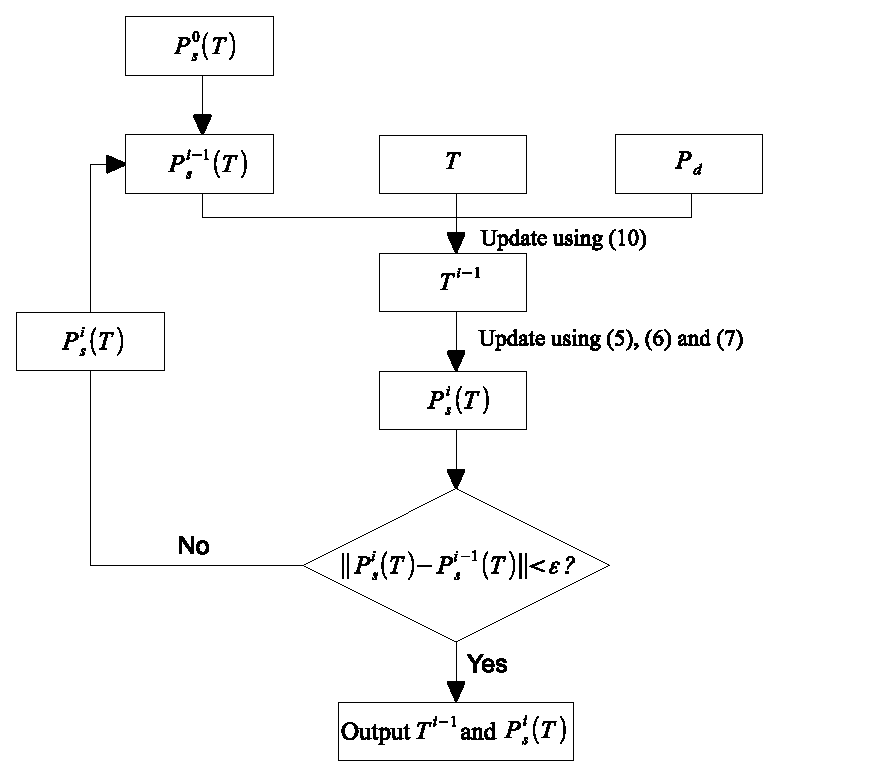
\includegraphics[width=1\linewidth]{fig/iteration_flow.eps}
\caption{Flow diagram of iteration based leakage-aware power estimation for one time step}
\end{figure}


Because of the dependency of static power on temperature, it's not straightforward to compute the static power and temperature of steady state based on current power. Iteration method can be implemented to solve such problem, the computation flow is shown in Fig.x.

The initial value of $P^0_s(T)$ is a guess we provide based on the process technology. The temperature distribution $T^0$ can be calculated with such guess. $P^1_s(T)$, the static power of next time step is updated with $T^0$. Next, the temperature distribution $T^1$ can be derived from $P^1_s(T)$, which concludes one iteration loop. Such iteration goes on until the convergence test is satisfied as $\| P^i_s(T)$-$P^(i-1)_s(T)\|<\epsilon$. Finally, the static power and temperature of steady state is outputted.

Combined with the brute force search static, the iteration based power estimation method can produce an accurate outcome providing the $\epsilon$ is chosen to be small enough, which could be considered as the golden accuracy baseline. However, the simulation time for such iteration based method is way too long, especially for multi-core systems with a large core number. 


\begin{figure*}[htb]
\centering
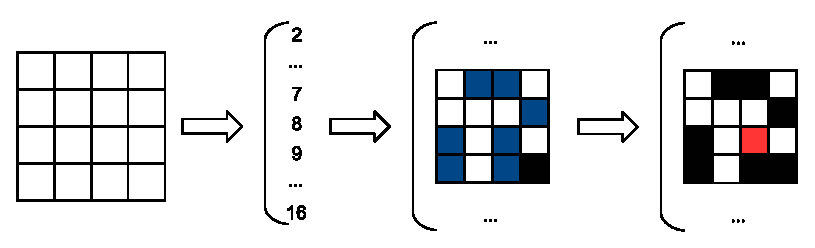
\includegraphics[width=0.8\textwidth]{fig/greedy_method.eps}
\caption{some figure}
\end{figure*}


\subsection{Local linearized thermal model}
The major difficulty of calculating leakage-aware power estimation comes from the nonlinear thermal model shown in (x), which is caused by the nonlinear relation between subthreshold current and temperature.To reduce the long computing time caused by iteration method, the leakage current $I_{leak}$ can be linearized to eliminate the non-linearity between $p_{s}$ and temperature, thus accelerating the computation. The basic idea is to approximate the original nonlinear leakage model using multiple new linear leakage models. By implementing such linear leakage models, we can reformulate the original nonlinear thermal model into multiple linear thermal models, such that traditional non-iteration based thermal estimation method can be applied.

In order to generate a linear leakage model, Taylor expansion is performed on the original $I_{leak}$ model at a expansion point $T_{0}$. Thus the linearized relation of $I_{leak}$ and temperature is obtained as:
\begin{equation}\label{linear_subthreshold}
\begin{split}
I_{sub} = &K(\frac{k}{q})^{2}e^(\frac{q(V_{GS}-V{th})}{\eta kT_{p0}}\\
&\times (T_{p0}^{2}+(2T_{p0}-\frac{q(V_{GS}-V_{th})}{\eta k})(T_{p}-T_{p0}))\\
&+ o[(T_{p}-T_{p0})^{2}],
\end{split}
\end{equation}
where $o[(T_{p}-T_{p0})^{2}]$ is the remainder. By ignoring the remainder, the linearized $I_{sub}$, denoted as $I_{lin}$ can be expressed as:
\begin{equation}\label{linear_subthreshold}
\begin{split}
I_{lin} = &K(\frac{k}{q})^{2}e^(\frac{q(V_{GS}-V{th})}{\eta kT_{p0}}\\
&\times (T_{p0}^{2}+(2T_{p0}-\frac{q(V_{GS}-V_{th})}{\eta k})(T_{p}-T_{p0})).
\end{split}
\end{equation}

Provided the actual temperature value $T_{p}$ is close to the reference temperature point $T_{p0}$, the approximation accuracy of $I_{lin}$ can be guaranteed. From previous research, it has been shown that due to the characteristic of today's semiconductor process, such local linear approximation of leakage current has high accuracy around the expansion point.

With the linearized relation of subthreshold current and temperature, the relation between static power and temperature in linear form can also be achieved as:
\begin{equation}\label{linear_static}
\begin{split}
p_{s} &= V_{dd}I_{leak}\\
&= V_{dd} \times (I_{lin}+I_{gate})\\
&= V_{dd} \times (I_{lin}(T_{p})+I_{const}),
\end{split}
\end{equation}
where $I_{lin}(T_{p})$ represents the terms associated with $T_{p}$ in (x), $I_{const}$ contains constant terms that are not associated with $T_{p}$ and the gate leakage $I_{gate}$.

A new linear thermal model can be built based on this static power model. In order to do that, we need to integrate (x) into (x). Please note that (x) is in scalar form for only one certain thermal node while (5) is in vector/matrix form including information of all thermal nodes. Therefore, by collecting and accumulating scalars $I_{lin}(T_{p})$ and $I_{const}$ at multiple positions of the chip into vectors, we can rewrite (x) in vector/matrix form. The current variables can also be changed to power by multiplying voltage $V_{dd}$. The linearized static power equation in matrix form is
\begin{equation}\label{linear_static_matrix}
P_{s} = P_{0}+A_{s}T
\end{equation}
where $P_{0} \in \mathbb{R}^{l}$ is a known vector, with each element formed by terms not associated with $T_{p}$ in (x) at each position of the chip. $A_{s} \in \mathbb{R}^{l \times n}$ is a known rectangular diagonal matrix (the left $l \times l$ block matrix is diagonal representing thermal nodes on the chip, and the right $l \times (n-l)$ block matrix is all zeros representing the thermal nodes of packages), with each diagonal element formed by the coefficient associated with $T_{p}$ in (x) at each position of the chip.

Integrating (14) into (8), and let $G_{l} = G - BA_{s}$, we have

\begin{equation}\label{gt=bp}
G_{l}T(t) + C\frac{dT(t)}{dt} = B(P_{d} + P_{0})
\end{equation}

With the obtained linear thermal model considering static power and eliminated the nonlinear relationship of static power and temperature, we can simulate the locally linearized leakage-aware thermal model just as in (8) by viewing "$G_{l}$" as the new "$G$" matrix and "$P_{d} + P_{0}$" as the new "$P_{T}$" vector.

\subsection{Non-iteration based power estimation}
Since we have generated the linearized thermal model as shown above, the Taylor expansion temperature points need to be determined, for they affect the linearized thermal model's accuracy greatly, also $P_{0}$ and $A_{s}$ in (14) are formulated by the expansion point information. Therefore, we will discuss how to determine the Taylor expansion points for thermal nodes in the system. 

As a property of Taylor expansion approximation, it is accurate only when the actual temperature $T_{p}$ is close to the expansion point $T_{p0}$. As a result, in order to ensure the approximation accuracy, we want each expansion point $T_{p0}$ to be close to the actual temperature $T_{p}$. To find a totally accurate outcome, $T_{p} = T_{p0}$ is necessary. However, such strategy requires $T_{p0}$ to be updated for each iteration, which would lead to much longer computing time than we expected. In order to balance the accuracy and computing time, the remainder $o[(T_{p}-T_{p0})^{2}]$ introduced by the deviation of $T_{p0}$ from $T_{p}$ can be tolerated if $T_{p0}$ is not far from $T_{p}$.

Considering that the temperature difference between the idle cores and active cores can be very large, it's not possible to find a single Taylor expansion temperature point that produces remainder $o[(T_{p}-T_{p0})^{2}]$ within tolerance for idle cores and active cores simultaneously.

In this work, we can notice that the temperature of cores can be classified into two parts, one is for active-state cores around \SI{70}{\degreeCelsius}, one is for idle-state cores around \SI{40}{\degreeCelsius}. Therefore, in order to balance the accuracy and computing cost, we set two Taylor expansion temperature points $T_{p1}$ and $T_{p2}$, one for active cores, one for idle cores. As can be shown in the experimental results, the approximation accuracy of this strategy is satisfactory in this work.




\subsection{Greedy search static based acceleration of light core distribution estimation}
In previous sections, to find the optimal light core distribution for a multi-core system which leads to highest performance-per-watt, a combinational method with high complexity is implemented. However, it's  especially impractical when the number of cores is too large. It is also noticed that for such systems, finding the optimal solution is not necessary. This is due to the fact that when core number is large, each core takes relatively small area, so there exist many sub-optimal active core distributions which only have slightly larger objective values (measured by cost function) than that of the optimal solution. Therefore, a greedy based method which can find a sub-optimal light core distribution with much less time consumption is applied. 

Since a sub-optimal solution may have only slightly worse performance compared with the optimal solution, instead of finding the optimal solution using combinational method with high complexity, we seek for a fast method to find a sub-optimal solution.

For a $n$-core system with $n_{a}$ light cores, the basic idea of finding such sub-optimal light core distribution is described as follows: we first find the optimal solution for only one light core. Next, we fix the first light core position determined by the first step, and find the optimal solution of two cores, with the second light core position determined. Please note that although we say “optimal” in the second step, such solution is only the optimal solution with the first light core fixed at the position determined by the first step, but not the true optimal solution for general two light cores. Similarly, in the ($i$ + 1)-th step, we look for the optimal solution for $i$ + 1 light cores with the positions of $i$ light cores found in all previous steps remain fixed. This process is shown in Fig. x. By proceeding such strategy for $n$ steps, the optimum light core number that leads to maximum PPW can be specified.
